
\documentclass[a4paper,11pt]{article}
\usepackage[a4paper, margin=8em]{geometry}

% usa i pacchetti per la scrittura in italiano
\usepackage[french,italian]{babel}
\usepackage[T1]{fontenc}
\usepackage[utf8]{inputenc}
\frenchspacing 

% usa i pacchetti per la formattazione matematica
\usepackage{amsmath, amssymb, amsthm, amsfonts}

% usa altri pacchetti
\usepackage{gensymb}
\usepackage{hyperref}
\usepackage{standalone}

% imposta il titolo
\title{Appunti Elettronica Digitale}
\author{Luca Seggiani}
\date{2026}

% imposta lo stile
% usa helvetica
\usepackage[scaled]{helvet}
% usa palatino
\usepackage{palatino}
% usa un font monospazio guardabile
\usepackage{lmodern}

\renewcommand{\rmdefault}{ppl}
\renewcommand{\sfdefault}{phv}
\renewcommand{\ttdefault}{lmtt}

% disponi il titolo
\makeatletter
\renewcommand{\maketitle} {
	\begin{center} 
		\begin{minipage}[t]{.8\textwidth}
			\textsf{\huge\bfseries \@title} 
		\end{minipage}%
		\begin{minipage}[t]{.2\textwidth}
			\raggedleft \vspace{-1.65em}
			\textsf{\small \@author} \vfill
			\textsf{\small \@date}
		\end{minipage}
		\par
	\end{center}

	\thispagestyle{empty}
	\pagestyle{fancy}
}
\makeatother

% disponi teoremi
\usepackage{tcolorbox}
\newtcolorbox[auto counter, number within=section]{theorem}[2][]{%
	colback=blue!10, 
	colframe=blue!40!black, 
	sharp corners=northwest,
	fonttitle=\sffamily\bfseries, 
	title=~\thetcbcounter: #2, 
	#1
}

% disponi definizioni
\newtcolorbox[auto counter, number within=section]{definition}[2][]{%
	colback=red!10,
	colframe=red!40!black,
	sharp corners=northwest,
	fonttitle=\sffamily\bfseries,
	title=~\thetcbcounter: #2,
	#1
}

% U.D.M
\newcommand{\amp}{\ensuremath{\mathrm{A}}}
\newcommand{\volt}{\ensuremath{\mathrm{V}}}
\newcommand{\meter}{\ensuremath{\mathrm{m}}}
\newcommand{\second}{\ensuremath{\mathrm{s}}}
\newcommand{\farad}{\ensuremath{\mathrm{F}}}
\newcommand{\henry}{\ensuremath{\mathrm{H}}}
\newcommand{\siemens}{\ensuremath{\mathrm{S}}}

% circuiti
\usepackage{circuitikz}
\usetikzlibrary{babel}

% disegni
\usepackage{pgfplots}
\pgfplotsset{width=10cm,compat=1.9}

% disponi codice
\usepackage{listings}
\usepackage[table]{xcolor}

\definecolor{codegreen}{rgb}{0,0.6,0}
\definecolor{codegray}{rgb}{0.5,0.5,0.5}
\definecolor{codepurple}{rgb}{0.58,0,0.82}
\definecolor{backcolour}{rgb}{0.95,0.95,0.92}

\lstdefinestyle{codestyle}{
		backgroundcolor=\color{black!5}, 
		commentstyle=\color{codegreen},
		keywordstyle=\bfseries\color{magenta},
		numberstyle=\sffamily\tiny\color{black!60},
		stringstyle=\color{green!50!black},
		basicstyle=\ttfamily\footnotesize,
		breakatwhitespace=false,         
		breaklines=true,                 
		captionpos=b,                    
		keepspaces=true,                 
		numbers=left,                    
		numbersep=5pt,                  
		showspaces=false,                
		showstringspaces=false,
		showtabs=false,                  
		tabsize=2
}

\lstdefinestyle{shellstyle}{
		backgroundcolor=\color{black!5}, 
		basicstyle=\ttfamily\footnotesize\color{black}, 
		commentstyle=\color{black}, 
		keywordstyle=\color{black},
		numberstyle=\color{black!5},
		stringstyle=\color{black}, 
		showspaces=false,
		showstringspaces=false, 
		showtabs=false, 
		tabsize=2, 
		numbers=none, 
		breaklines=true
}

\lstdefinelanguage{javascript}{
	keywords={typeof, new, true, false, catch, function, return, null, catch, switch, var, if, in, while, do, else, case, break},
	keywordstyle=\color{blue}\bfseries,
	ndkeywords={class, export, boolean, throw, implements, import, this},
	ndkeywordstyle=\color{darkgray}\bfseries,
	identifierstyle=\color{black},
	sensitive=false,
	comment=[l]{//},
	morecomment=[s]{/*}{*/},
	commentstyle=\color{purple}\ttfamily,
	stringstyle=\color{red}\ttfamily,
	morestring=[b]',
	morestring=[b]"
}

% disponi sezioni
\usepackage{titlesec}

\titleformat{\section}
	{\sffamily\Large\bfseries} 
	{\thesection}{1em}{} 
\titleformat{\subsection}
	{\sffamily\large\bfseries}   
	{\thesubsection}{1em}{} 
\titleformat{\subsubsection}
	{\sffamily\normalsize\bfseries} 
	{\thesubsubsection}{1em}{}

% disponi alberi
\usepackage{forest}

\forestset{
	rectstyle/.style={
		for tree={rectangle,draw,font=\large\sffamily}
	},
	roundstyle/.style={
		for tree={circle,draw,font=\large}
	}
}

% disponi algoritmi
\usepackage{algorithm}
\usepackage{algorithmic}
\makeatletter
\renewcommand{\ALG@name}{Algoritmo}
\makeatother

% disponi numeri di pagina
\usepackage{fancyhdr}
\fancyhf{} 
\fancyfoot[L]{\sffamily{\thepage}}

\makeatletter
\fancyhead[L]{\raisebox{1ex}[0pt][0pt]{\sffamily{\@title \ \@date}}} 
\fancyhead[R]{\raisebox{1ex}[0pt][0pt]{\sffamily{\@author}}}
\makeatother

\begin{document}
% sezione (data)
\section{Lezione del 31-03-26}

% stili pagina
\thispagestyle{empty}
\pagestyle{fancy}

% testo
\subsubsection{Analisi dell'amplificatore ad emettitore comune}
Siamo quindi pronti ad effettuare un analisi vera e propria dell'amplificatore ad emettitore comune. Lo avevamo introdotto in 11.2.2 parlando di amplificatori e dell'accoppiamento termico dei BJT; quindi lo avevamo ripreso nella scorsa lezione per parlare dell'accoppiamento AC. Adesso proviamo effettivamente a studiarlo come circuito non lineare nei regimi di operazione AC e DC.

\newpage

Il circuito da studiare sarà quindi il seguente, dove notiamo dell'aggiunta della capacità ad emettitore $C_E$ (la sua motivazione ci sarà chiara a breve):
\begin{center}
\begin{circuitikz}
	\draw
(0,0) node[ground]{} to[R=$R_2$] (0,3)
to[R=$R_1$] (0,6) node[vcc]{};

\draw (0,3) -- (2,3);

\draw (2,3) node[npn, anchor=B] (Q1) {};

\draw (Q1.C) to[R=$R_C$] ++(0,3) node[vcc]{};
\draw (Q1.E) to[R=$R_E$] ++(0,-3) node[ground]{};

\draw[->] (1.2,3.3) -- (1.8,3.3) node[midway, above]{$I_B$};
\draw[->] (Q1.C) ++(0.3,0.5) -- ++(0,-1) node[midway, right]{$I_C$};
\draw[->] (Q1.E) ++(0.3,0) -- ++(0,-.8) node[midway, right]{$I_E$};

\node[ground] at(-4, 0) {};
\draw (-4, 0) to [ sinusoidal voltage source, v=$V_s$] (-4,3)
	to [resistor, l=$R_s$] (-2, 3)
	to [capacitor, l=$C_s$] (0, 3);

\node[ground] at(6, 0) {};
\draw(3, 4.5) to[ capacitor, l=$C_L$] (6, 4.5)
	to[resistor, l=$R_L$] (6, 0);

\draw(2.8, 0) -- (2, 0) to[capacitor, l=$C_E$] (2, 1.5) -- (2.8, 1.5);

\end{circuitikz}
\end{center}

Notiamo che faremo due trattazioni:
\begin{itemize}
	\item La prima prenderà considererà la capacità di accoppiamento $C_E$ all'emettitore, e mostrerà come questa aumenta la capacità di amplificazione del circuito;
	\item La seconda invece non la considererà, e mostrerà come questo riduce l'amplificazione effettiva.
\end{itemize}

\par\smallskip

\noindent
\textbf{\textsf{Con capacità di accoppiamento}}

\noindent
Consideriamo la componente DC già calcolata col punto di quiescenza determinato dal bias di $R_1$ e $R_2$. In questo caso potremo passare all'analisi AC considerare tutte le capacità di accoppiamento come cortocicuito, inclusa quella ad $R_E$, e sostituire il transistor con il modello ai piccoli segnali. Avremo quindi l'impedenza di ingresso $h_{ie}$ e la sorgente di corrente pilotata in $h_{fe}$ da $i_b$ (per la legge $i_c = h_{fe} i_b$). Il circuito equivalente (cortesia della collega Imane Rajy) sarà:
\begin{center}
	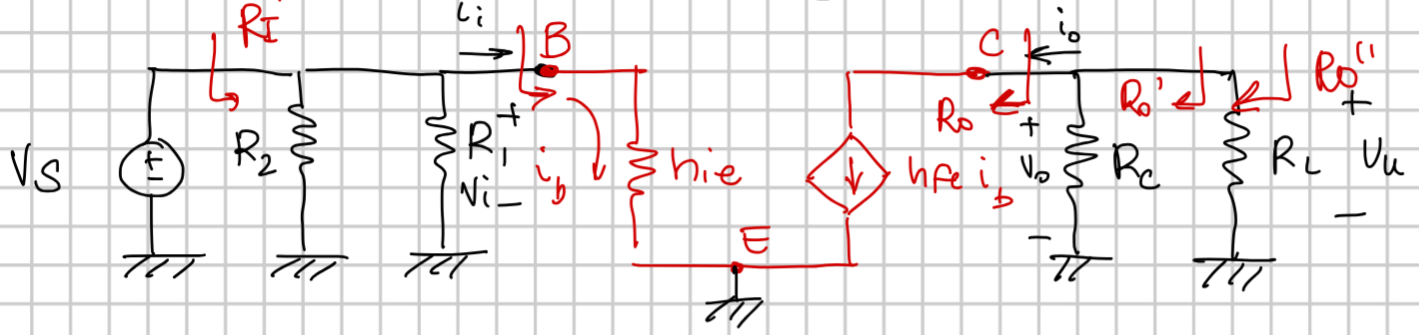
\includegraphics[scale=0.4]{../figures/trans_amp_imane_1.png}
\end{center}

Vogliamo calcolare i 4 parametri (guadagni di corrente e tensione, impedenze di ingresso e uscita) considerati per gli amplificatori in 11.2.1.

\begin{itemize}
\item \textbf{\textsf{Guadagno di corrente}} $A_i$ \\
Questo sarà immediato dalla corrente imposta all'uscita dal transistor, cioè:
$$
i_o = i_c = h_{fe} i_b
$$
e la corrente di ingresso, che con $R_E$ non considerata (dal corto su $C_E$ per segnali AC) consiste solamente in:
$$
i_i = i_b
$$

Il guadagno di corrente sarà quindi il rapporto:
$$
A_i = \frac{i_o}{i_i} = \frac{h_{fe} i_b}{i_b} = h_{fe}
$$
cioè il parametro $h_{fe}$, senza sorprenderci particolarmente, rappresenta il guadagno in corrente dell'amplificatore (come rappresentava il guadagno di corrente diretto del BJT stesso in parametri ibridi).

\item \textbf{\textsf{Guadagno di tensione}} $A_V$ \\
Per il guadagno di tensione avremo bisogno di un indicazione per la tensione in uscita all'amplificatore. Questa sarà data, ad esempio, dalla caduta su $R_C$ (trascurando la resistenza di carico $R_L$):
$$
v_o \Big|_{R_L \rightarrow +\infty} = - h_{fe} i_b R_C
$$
mentre le tensione in ingresso sarà semplicemente il segnale fornito:
$$
v_i = V_s
$$

Cerchiamo quindi una forma chiusa in $V_s$ della $v_o$ in modo da esprimere tutto in funzione di $V_s$ e ricavare un guadagno. Per fare ciò prendiamo la $i_b$ in funzione della $V_s$:
$$
i_b = \frac{V_s}{h_{ie}}
$$
e sostituiamo in $v_0$, da cui il guadagno:
$$
v_o = -h_{fe} R_C \frac{V_s}{h_{ie}}
\implies
A_V = -\frac{h_{fe} R_C}{h_{ie}}
$$

Notiamo qui una particolarità di questo tipo di amplificatore: abbiamo che è \textit{invertente} (il cosiddetto \textbf{inverting amplifier}), cioè la tensione in uscita è sfasata di $180^\circ$ rispetto alla tensione in entrata. Inoltre, notiamo che il guadagno calcolato è quello \textit{visto} all'uscita dell'amplificatore, posta la $R_L$ ad infinito (cioè come circuito aperto). Chiaramente collegando una resistenza di carico diversa si avrebbe un calo di tensione. 

\item \textbf{\textsf{Impedenza di uscita}} $R_o$ \\
Per calcolare l'impedenza di uscita si pone un generatore di prova $V_p$ all'uscita e si spenge il generatore di segnale $V_s$. A questo punto si può considerare la resistenza vista al collettore del transistore BJT, a valle della resistenza $R_C$, o a valle della resistenza $R_L$.

Al collettore del BJT si avrà, spento il generatore $V_s$, corrente $i_b$ nulla e di conseguenza corrente $i_c$ nulla, per cui in:
$$
R_o = \frac{v_o}{i_o} \Big|_{i_o \rightarrow 0} = + \infty
$$
cioè impedenza infinita.


Avremo quindi la sola $R_C$ nel caso in cui si consideri la resistenza alla $R_C$ in sé per sé, o dal parallelo:
$$
R_o = \frac{v_o}{i_o} = R_C || R_L
$$
nel caso in cui si consideri anche la resistenza di carico.

\item \textbf{\textsf{Impedenza di ingresso}} $R_i$ \\
L'impedenza di ingresso verrà calcolata in maniera simile, ponendo un generatore di prova al posto di $V_s$. In questo caso, visto che l'emettitore è collegato direttamente a massa, si avrà che tutto il lato destro del circuito è irrilevante al calcolo dell'impedenza in ingressso. Vedremo che togliendo la capacità $C_E$ questo non sarà più il caso. 

Prendiamo quindi il parallelo fra la resistenza associata al modello dei piccoli segnali del transistore, e le resistenze del partitore di bias $R_1$ e $R_2$:
$$
R_i = \frac{v_i}{i_i} = R_1 || R_2 || h_{ie} 
$$
\end{itemize}

Abbiamo quindi visto come introdurre la capacità di accoppiamento $C_E$ all'emettitore ci permette di avere disaccoppiamento in AC della resistenza $R_E$, e quindi semplificazioni nei calcoli e un aumento del guadagno di tensione. 

\par\smallskip

\noindent
\textbf{\textsf{Senza capacità di accoppiamento}}

\noindent
Vediamo adesso il caso con questa capacità rimossa, cioè preso il circuito:
\begin{center}
\begin{circuitikz}
	\draw
(0,0) node[ground]{} to[R=$R_2$] (0,3)
to[R=$R_1$] (0,6) node[vcc]{};

\draw (0,3) -- (2,3);

\draw (2,3) node[npn, anchor=B] (Q1) {};

\draw (Q1.C) to[R=$R_C$] ++(0,3) node[vcc]{};
\draw (Q1.E) to[R=$R_E$] ++(0,-3) node[ground]{};

\draw[->] (1.2,3.3) -- (1.8,3.3) node[midway, above]{$I_B$};
\draw[->] (Q1.C) ++(0.3,0.5) -- ++(0,-1) node[midway, right]{$I_C$};
\draw[->] (Q1.E) ++(0.3,0) -- ++(0,-.8) node[midway, right]{$I_E$};

\node[ground] at(-4, 0) {};
\draw (-4, 0) to [ sinusoidal voltage source, v=$V_s$] (-4,3)
	to [resistor, l=$R_s$] (-2, 3)
	to [capacitor, l=$C_s$] (0, 3);

\node[ground] at(6, 0) {};
\draw(3, 4.5) to[ capacitor, l=$C_L$] (6, 4.5)
	to[resistor, l=$R_L$] (6, 0);
\end{circuitikz}
\end{center}

In tal caso il circuito equivalente che otterremo in AC prevederà la resistenza $R_E$ all'emettitore del transistor, in quanto non potremmo semplificarla via col parallelo a $C_E$:
\begin{center}
	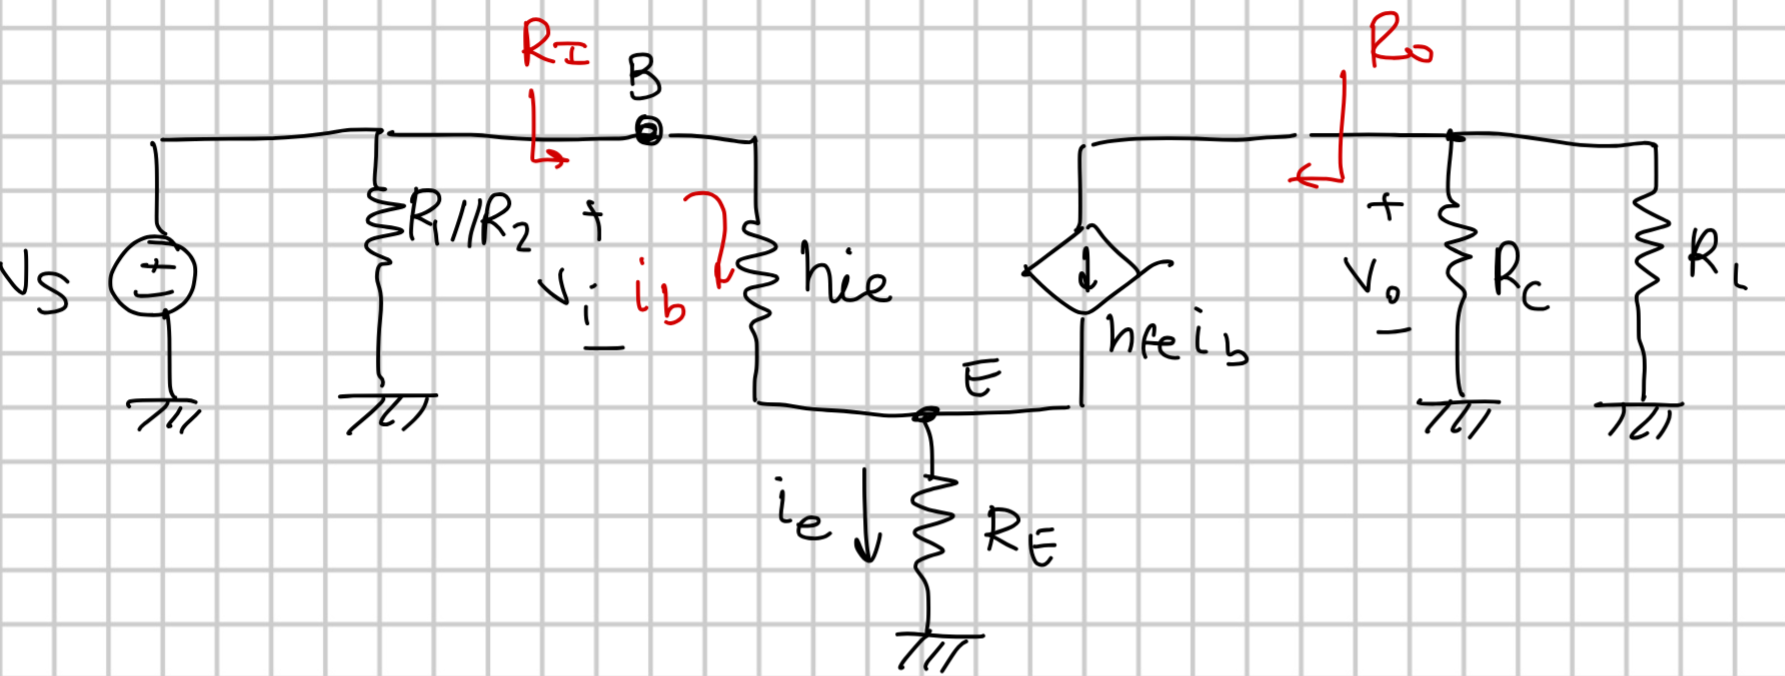
\includegraphics[scale=0.3]{../figures/trans_amp_imane_2.png}
\end{center}

Ricalcoliamo quindi gli stessi parametri dell'amplificatore, vedendo come variano.
\begin{itemize}
\item \textbf{\textsf{Guadagno di corrente}} $A_i$ \\
Questa non cambia, in quanto le correnti in entrata e in uscita restano le solite:
$$
i_i = i_b, \quad i_o = h_{fe} i_b
$$
da cui il guadagno corrente legato al parametro ibrido:
$$
A_i = \frac{i_o}{i_i} = \frac{h_{fe} i_b}{i_b} = h_{fe}
$$

\item \textbf{\textsf{Guadagno di tensione}} $A_V$ \\
	Cose più interessanti accadono per il guadagno di tensione. Abbiamo che non potremo calcolare solo la caduta sulla resistenza $h_{ie}$ all'ingresso, ma dovremmo tenere conto anche della caduta su $R_E$:
$$
v_i = h_{ie} i_b + V_E
$$
Le cose all'uscita restano invece uguali, cioè la tensione di uscita è:
$$
v_o \Big|_{R_L \rightarrow +\infty} = - h_{fe} i_b R_C
$$
preso come prima $R_L$ come un circuito aperto (tensione imposta a vuoto senza carichi resistivi).

Vediamo quindi come calcolare questa $V_E$. Questa dipenderà dalla corrente che passa su $R_E$ dalla prima legge di Kirchoff, cioè $i_b$ e $i_c = h_{fe} i_b$:
$$
V_E = (i_b + h_{fe} i_b) R_E
$$
per cui la $v_i$ totale (e di conseguenza il guadagno in tensione) risultano:
$$
v_i = i_b h_{ie} + (i_b + h_{fe}) R_e 
\implies
A_v = \frac{v_o}{v_i} \Big|_{R_L \rightarrow + \infty} 
$$
$$= - \frac{h_{fe} i_b R_C}{i_b i_e + (i_b + h_{fe} i_b) R_E} = - \frac{h_{fe} R_C}{h_{ie} + (1 + h_{fe}) R_E}
$$

Discutiamo questo risultato. L'amplificatore è sempre invertente, in quanto rimane il segno negativo. Si ha però una diminuzione del guadagno ottenuto dato dal componente:
$$
(1 + h_{fe}) R_E
$$
Ci potremmo chiedere come mai non includere sempre la capacità $C_E$ visto che questa aumenta il guadagno. La risposta è che, rimossa la $C_E$, e assunto $R_E$ sufficientemente grande, si ha approssimativamente:
$$
A_v = - \frac{h_{fe} R_C}{h_{ie} + (1 + h_{fe}) R_E} \sim -\frac{R_C}{R_E}
$$
cioè il calcolo del guadagno $A_v$ diventa triviale. In situazioni dove non è fondamentale ottenere un grande guadagno, ma piuttosto tararlo con precisione agendo su $R_E$ e $R_C$, e quindi più semplice non includere la capacità di accoppiamento $C_E$ e sfruttare l'approssimazione $\frac{R_C}{R_E}$ per il guadagno.

\item \textbf{\textsf{Impedenza di uscita}} $R_o$ \\
L'impedenza in uscita è esattamente analoga alla situazione vista con la capacità di accoppiamento $C_E$: si pone un generatore di prova $V_p$ all'uscita e si spenge il generatore di segnale $V_s$. A questo punto si può considerare la resistenza vista al collettore del transistore BJT, a valle della resistenza $R_C$, o a valle della resistenza $R_L$.

Al collettore del BJT si avrà, spento il generatore $V_s$, corrente $i_b$ nulla e di conseguenza corrente $i_c$ nulla, per cui di nuovo impedenza infinita.
Avremo quindi la sola $R_C$ nel caso in cui si consideri la resistenza alla $R_C$ in sé per sé, o dal parallelo: $R_C || R_L$ nel caso in cui si consideri anche la resistenza di carico.

\item \textbf{\textsf{Impedenza di ingresso}} $R_i$ \\
Veniamo quindi l'impedenza di ingresso, che avevamo anticipato risentiva dal lato uscita del circuito quando si rimuoveva la capacità di accoppiamento. Abbiamo infatti che ponendo il generatore di prova $V_p$ al posto di $V_s$ si ottiene la stessa identica corrente su $R_E$ (e quindi caduta $V_E$) che avevamo visto per il calcolo del guadagno in tensione. Risulta quindi che:
$$
V_p = h_{ie} i_p + (1 + h_{fe}) R_E i_p
$$
per cui l'impedenza vista è:
$$
R_i = \frac{V_p}{i_p} = h_{ie} + (1 + h_{fe}) R_E
$$
Questo è esattamente lo stesso termine trovato per il guadagno in tensione $A_v$, e ci mostra come è possibile che l'uscita del circuito influenzi l'impedenza vista all'ingresso. Chiamiamo la legge trovata \textbf{regola di riflessione della resistenza}. 

Infine notiamo che, chiaramente, questa impedenza viene calcolata prima elle resistenze $R_1$ e $R_2$. 

\end{itemize}
\end{document}
